\documentclass[a4paper,10pt,spanish,oneside]{article}

% Preámbulo - Parte A

\usepackage[utf8]{inputenc} % Soporte para los acentos
\usepackage[T1]{fontenc}

\usepackage[spanish]{babel} % Capítulos, seciones, etc. en español

\usepackage[margin=2cm]{geometry} % Diseño del documento

\usepackage{multicol} % Escribir doble columna

\usepackage{xcolor} % Usar colores
\usepackage{pstricks}

\usepackage{enumerate} % Cambiar etiquetas de numeración
\usepackage[shortlabels]{enumitem} % Manejo adicional de etiquetas de numeración

\usepackage{graphicx} % Manejo de gráficos y figuras

\usepackage{makeidx} % Índice alfabético

% Paquetes adicionales de símbolos matemáticos
\usepackage{amsmath,amssymb,amsfonts,latexsym,cancel} 

% \usepackage{pslatex} % Fuente Times
% \usepackage{mathpazo} % Fuente Palatino
% \usepackage{mathptmx} % Fuente Times
% \usepackage{bookman} % Fuente Bookman
\usepackage{newcent} % Fuente New Century Schoolbook
% \usepackage{helvet} % Fuente Helvetica
% \usepackage{palatino} % Fuente Palatino
% \usepackage{pxfonts} % Fuente 
% \usepackage{txfonts} % Fuente
% \usepackage{concrete} % Fuente
% \usepackage{cmbright} % Fuente
% \usepackage{fourier} % Fuente

\usepackage{booktabs} % Opciones adicionales para el entorno tabular
\usepackage{longtable} % Para tablas de más de una página

\usepackage{tikz} % Creación de gráficos

% \usepackage{titlesec} % Personalizar capítulos y secciones

% Preámbulo - Parte B

\pagestyle{headings}

%\pagestyle{myheadings} % Numeración de página en la parte superior

\usepackage{titlesec}

\titleformat{\section} % command
			[display] % shape
			{\usefont{T1}{phv}{b}{n}\LARGE} % format
			{} % label
			{1pt} % sep
			{\thesection.\hspace{0.5em}} % before code
			
\titleformat{\subsection} % command
			[display] % shape
			{\usefont{T1}{phv}{b}{n}\Large} % format
			{} % label
			{1pt} % sep
			{\thesubsection.\hspace{0.5em}} % before code
			
\titleformat{\subsubsection} % command
			[display] % shape
			{\usefont{T1}{phv}{b}{n}\large} % format, fuentes: lmss,pag,phv
			{} % label
			{1pt} % sep
			{\thesubsubsection.\hspace{0.5em}} % before code		

\titleformat{name=\section,numberless}
			[display]
			{\usefont{T1}{phv}{b}{n}\LARGE}
			{}
  			{1pt}
  			{}
			\titlespacing*{\section}{0pt}{1pt}{1pt}

%---
\usepackage{geometry} %Algo de las líneas del pie y encabezados
\geometry{text={7in,9.5in},headheight=15pt}
%\textwidth = 7 in
%\textheight = 9.5 in
%\oddsidemargin = -0.25 in
%\evensidemargin = 0.0 in
%\topmargin = -0.25 in
%\headheight = 0.0 in
%\headsep = 0.0 in
\setlength{\parskip}{0.1in}
\setlength{\parindent}{0.0in}
%---
\usepackage{fancyhdr} %Para usar encabezados y pies personalizados
	\pagestyle{fancy}
	\fancyhf{}
	\fancyhead[LE,RO]{Tecnologías para la Web Semántica} 
	\fancyhead[RE,LO]{Protégé}
	\fancyfoot[RE,LO]{Darién Julián Ramírez}
	\fancyfoot[LE,RO]{\thepage}
	\renewcommand{\footrulewidth}{1pt}
%---
\usepackage{listings} %Para escribir códigos
\lstset{language=XML,
	basicstyle=\footnotesize,
	numbers=left,
 	stepnumber=1,
	numbersep=8pt,
	showspaces=false,               % show spaces adding particular underscores
  	showstringspaces=false,         % underline spaces within strings
  	frame=lines,                   % adds a frame around the code
	tabsize=4,                      
  	captionpos=b,                   % sets the caption-position to bottom
  	breaklines=true,                % sets automatic line breaking
}
%---

% Preámbulo - Parte B

\title{\Huge\usefont{T1}{}{}{n} Tecnologías para la Web Semántica\\
									 Trabajo Práctico Nº8\\
									 Protégé}
\author{Darién Julián Ramírez}
\date{}

% Cuerpo del documento

\begin{document}

\maketitle % Mostrar título

\begin{minipage}{0.3\linewidth}

Para la construcción de la ontología con \textit{Protégé} lo primero que se debe hacer es comenzar a crear las clases correspondientes al modelo diseñado. Todas las clases creadas serán subclases de una clase llamada \textit{Thing}. Todas estás clases creadas, de momento, no se encuentran relacionadas. Dichas relaciones se establecerán después pero para ello primero se deben definir las \textit{Object properties}.

\end{minipage} \hfill \begin{minipage}{0.65\linewidth}

\begin{center}
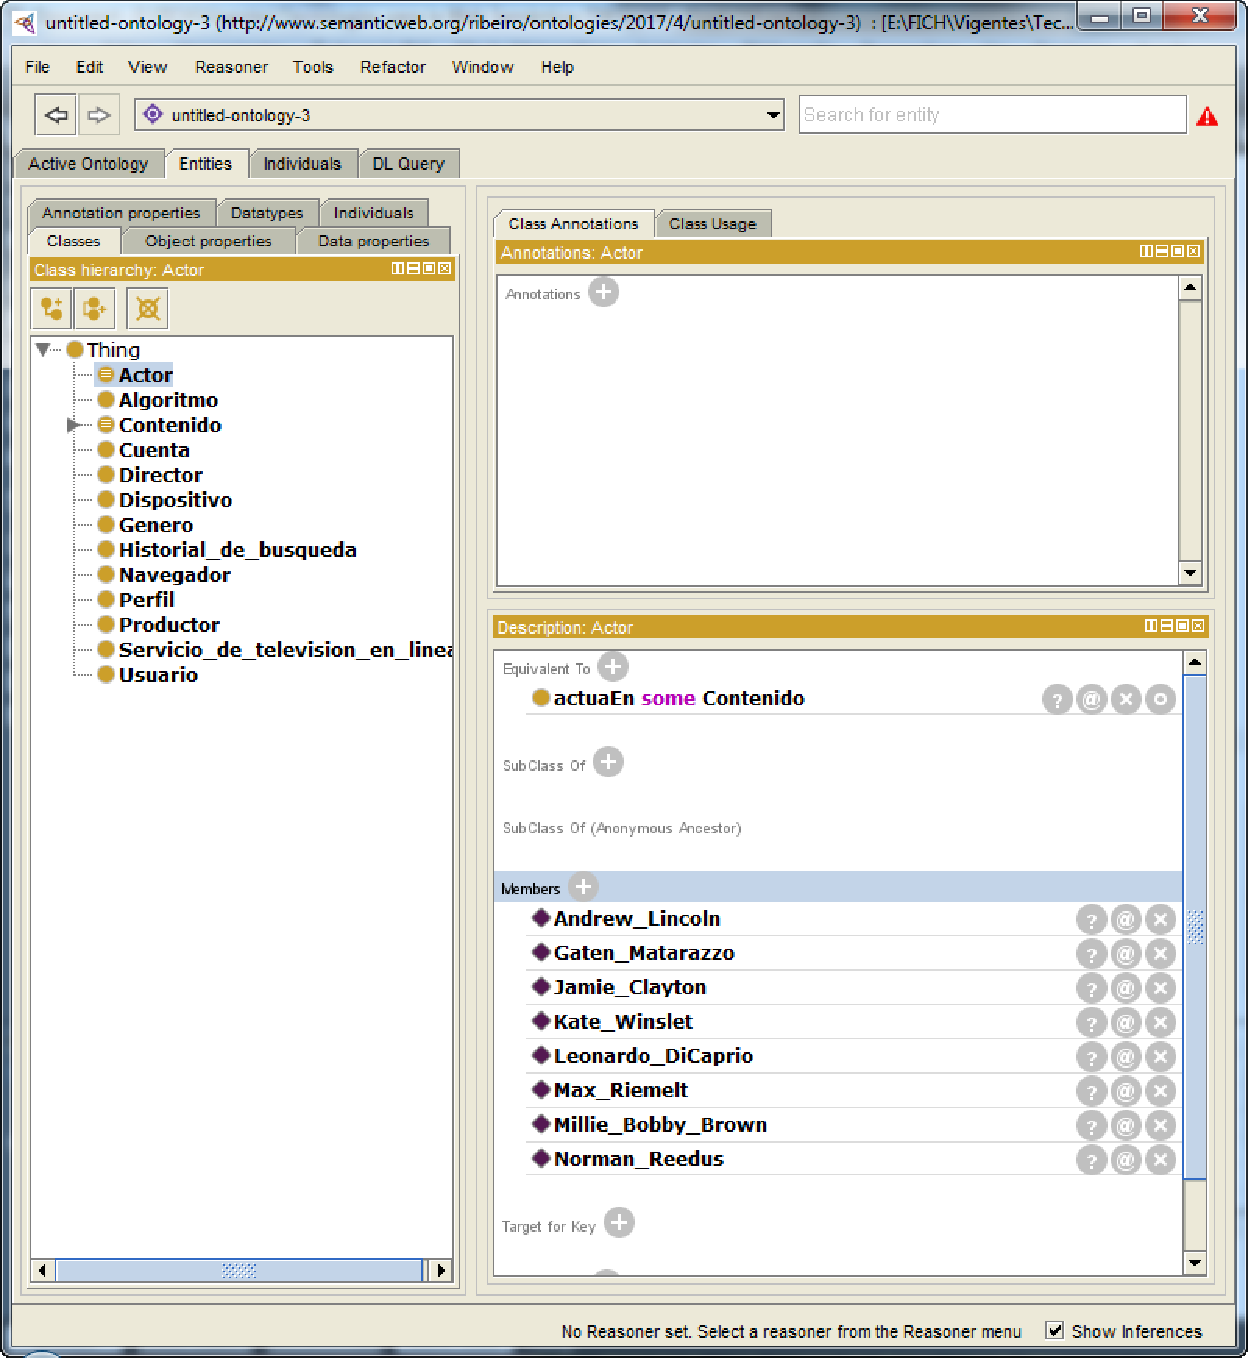
\includegraphics[width=\linewidth]{1}
\end{center}

\end{minipage}

\begin{minipage}{0.3\linewidth}

Se cargan cada una de las relaciones (\textit{Object properties}) que vinculan a las clases de la ontología pero por el momento no se determinan los dominios y rangos de cada una de ellas.

\end{minipage} \hfill \begin{minipage}{0.65\linewidth}

\begin{center}
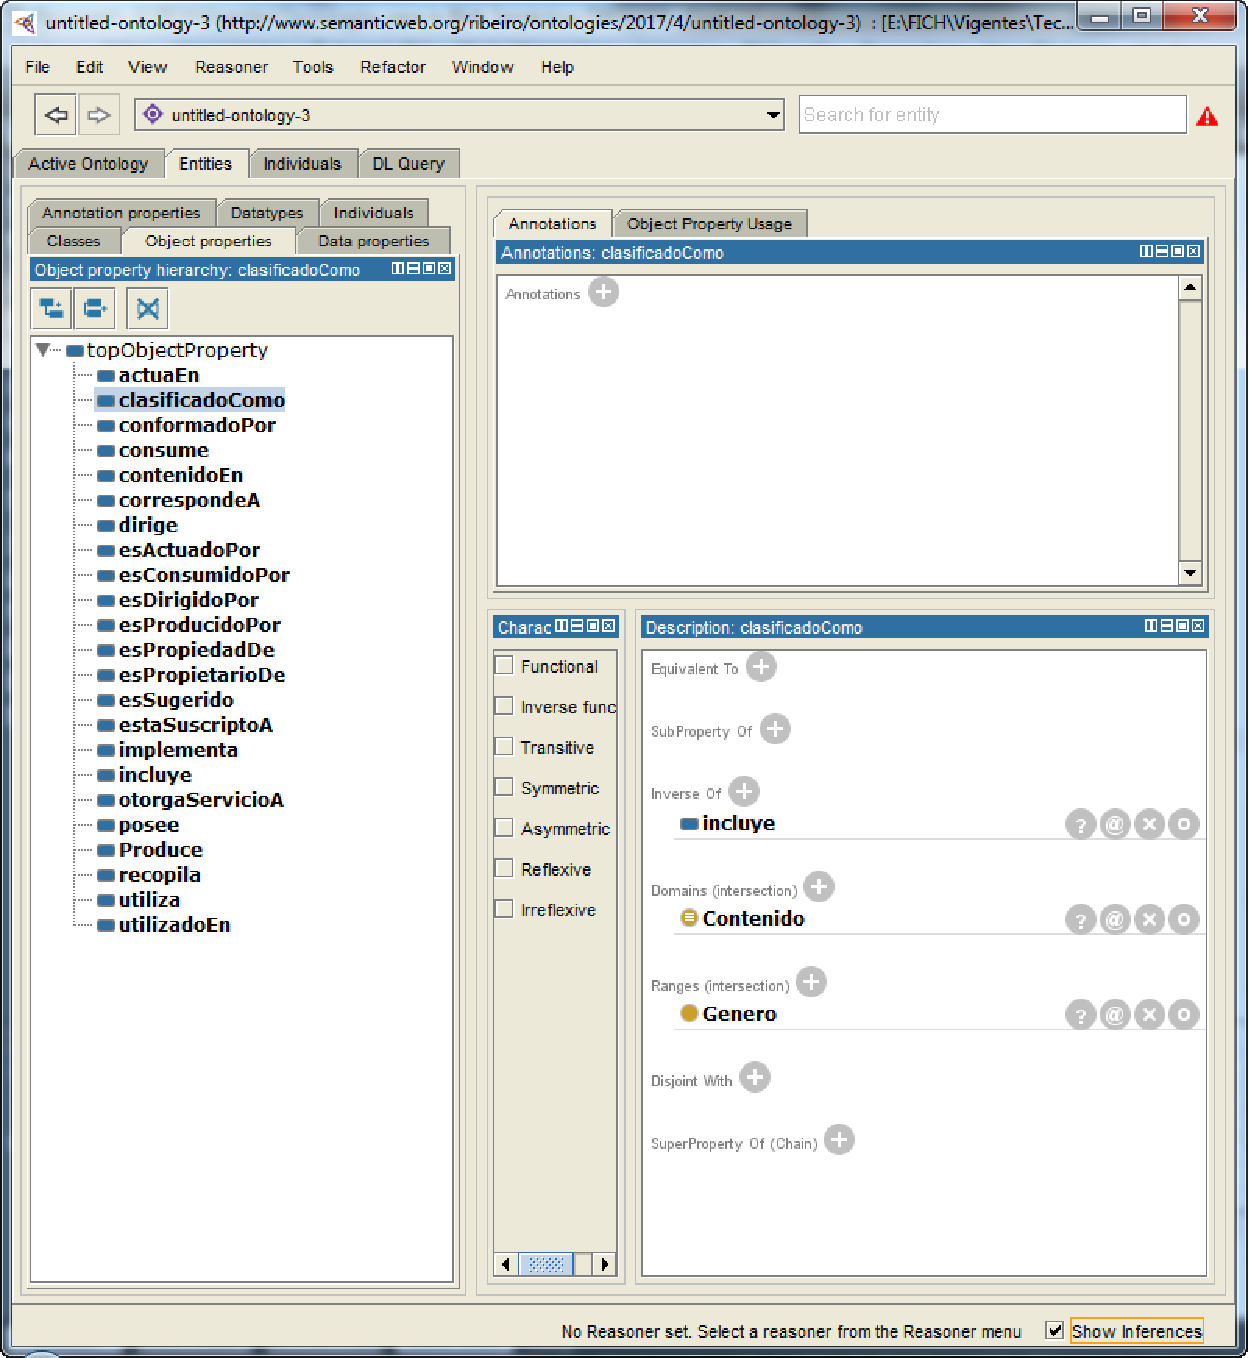
\includegraphics[width=\linewidth]{2}
\end{center}

\end{minipage}

\begin{minipage}{0.3\linewidth}

Ahora se cargan los atributos de las clases (\textit{Data properties}) que posteriormente serán asignados.

\end{minipage} \hfill \begin{minipage}{0.65\linewidth}

\begin{center}
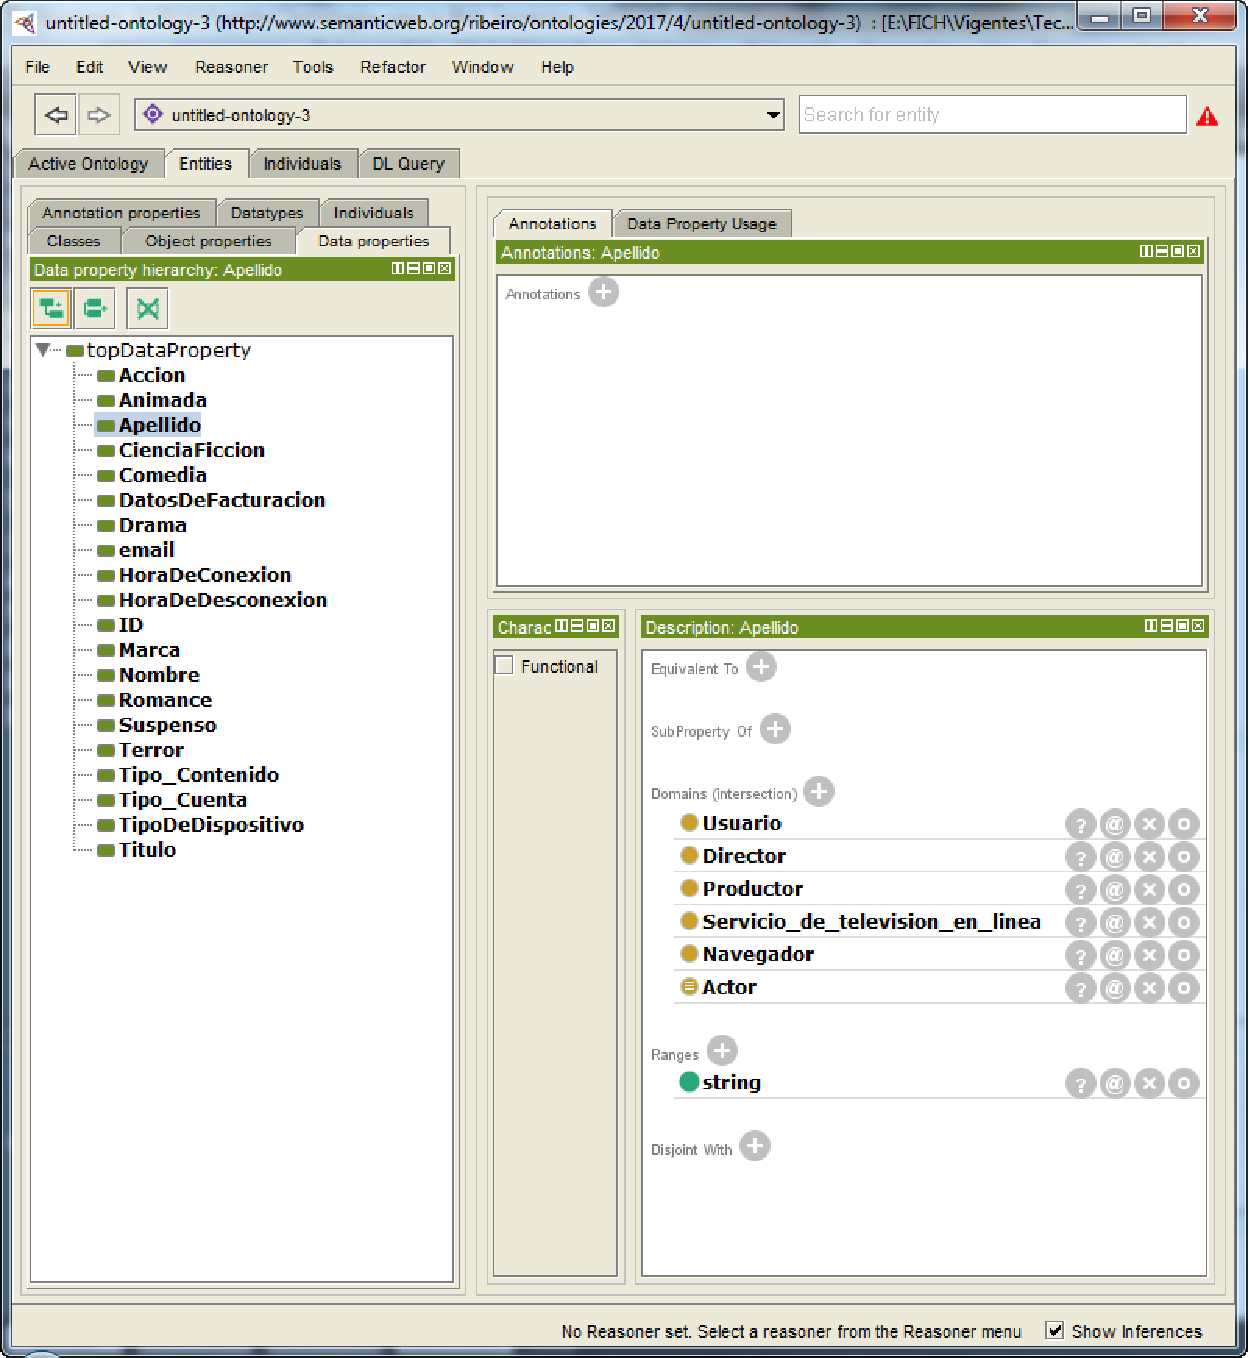
\includegraphics[width=\linewidth]{3}
\end{center}

\end{minipage}

\begin{minipage}{0.3\linewidth}

Se pasa a cargar las instancias del modelo. Para cada una de las clases de la ontología planteada se generan instanciaciones.

\end{minipage} \hfill \begin{minipage}{0.65\linewidth}

\begin{center}
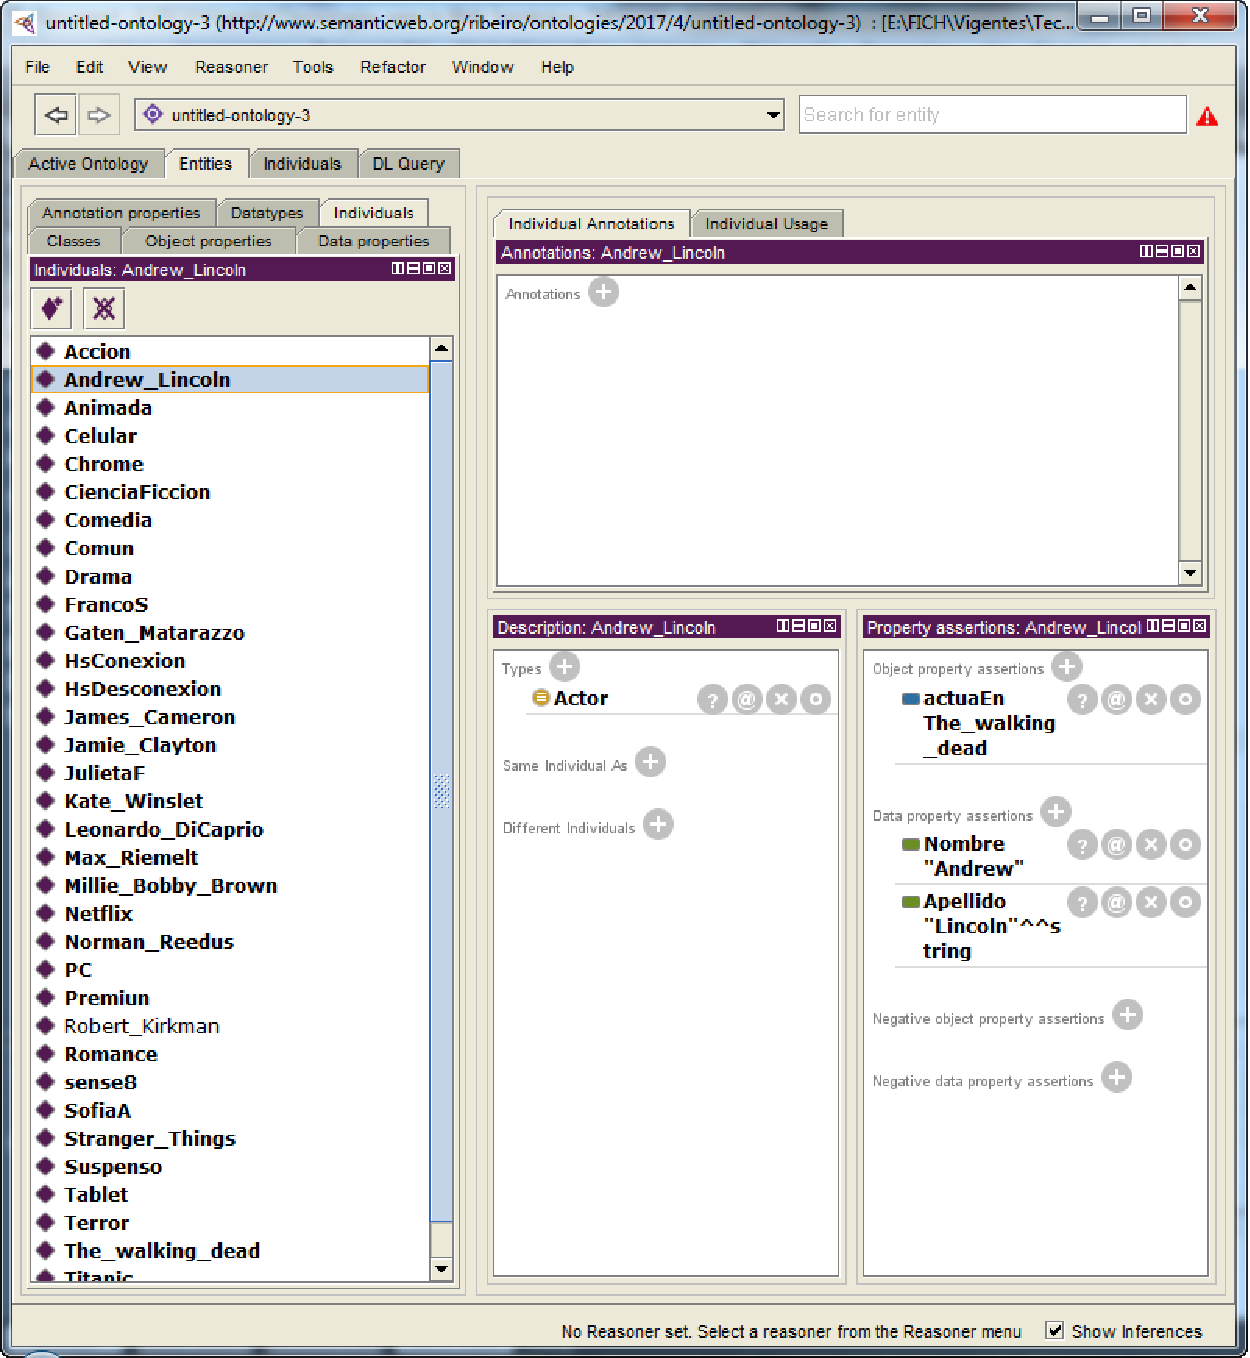
\includegraphics[width=\linewidth]{4}
\end{center}

\end{minipage}

\begin{minipage}{0.3\linewidth}

Se comienzan a establecer los dominios y rangos de las relaciones, las tripletas, a través de la opción \textit{Equivalente to}. A partir de éstas acciones, las \textit{Object properties} ya se irán completando también.

\end{minipage} \hfill \begin{minipage}{0.65\linewidth}

\begin{center}
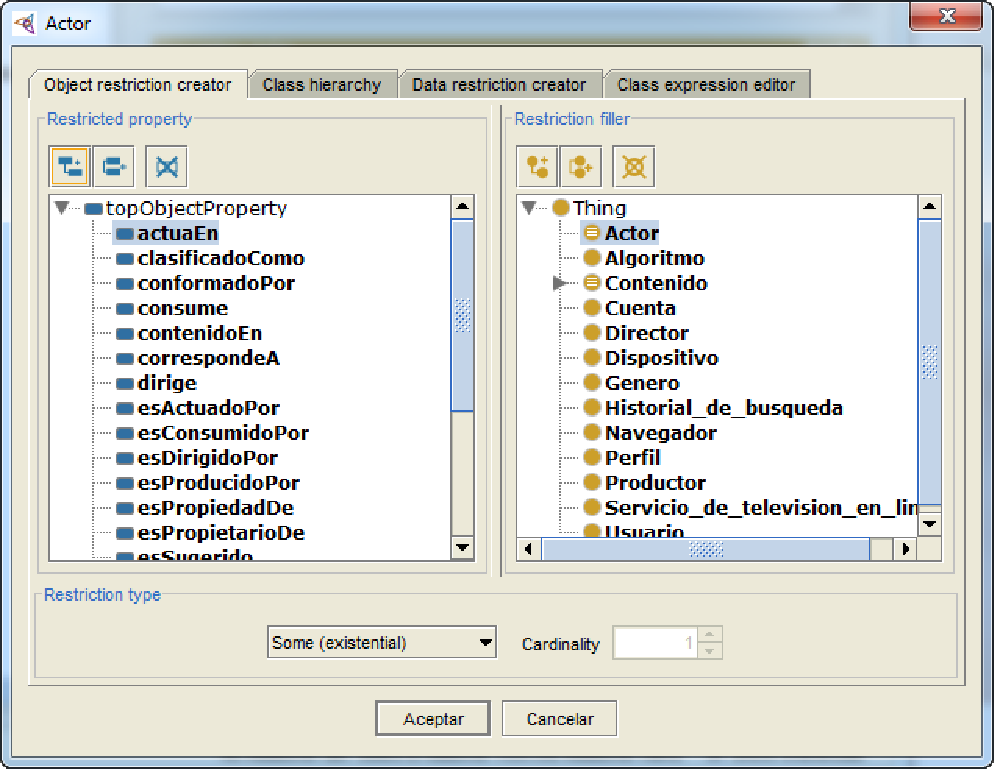
\includegraphics[width=\linewidth]{5}
\end{center}

\end{minipage}

\begin{minipage}{0.3\linewidth}

Además se agregan también las instancias correspondientes a cada clase mediante la opción \textit{Members}.

\end{minipage} \hfill \begin{minipage}{0.65\linewidth}

\begin{center}
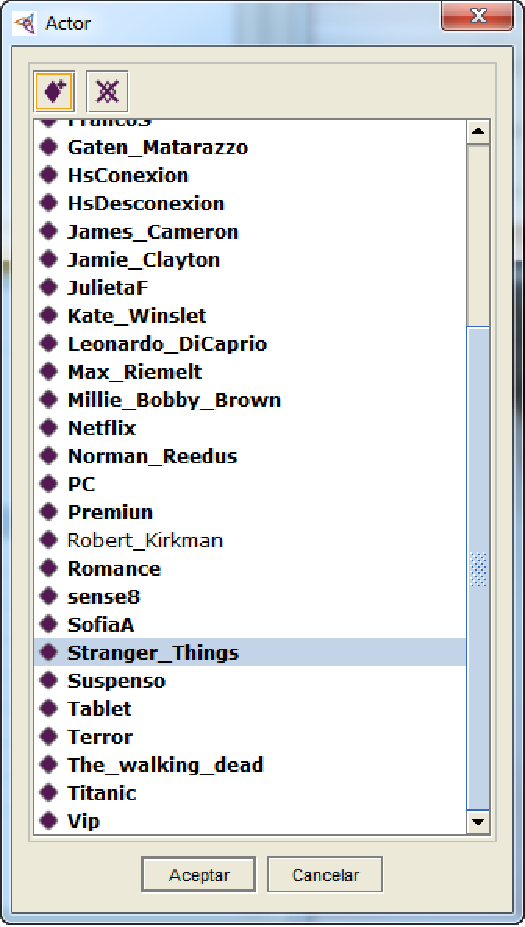
\includegraphics[width=0.5\linewidth]{6}
\end{center}

\end{minipage}

\begin{minipage}{0.3\linewidth}

Para las \textit{Object properties} además, deben agregarse en caso de ser necesario las relaciones inversas, las subclases, etc.

\end{minipage} \hfill \begin{minipage}{0.65\linewidth}

\begin{center}
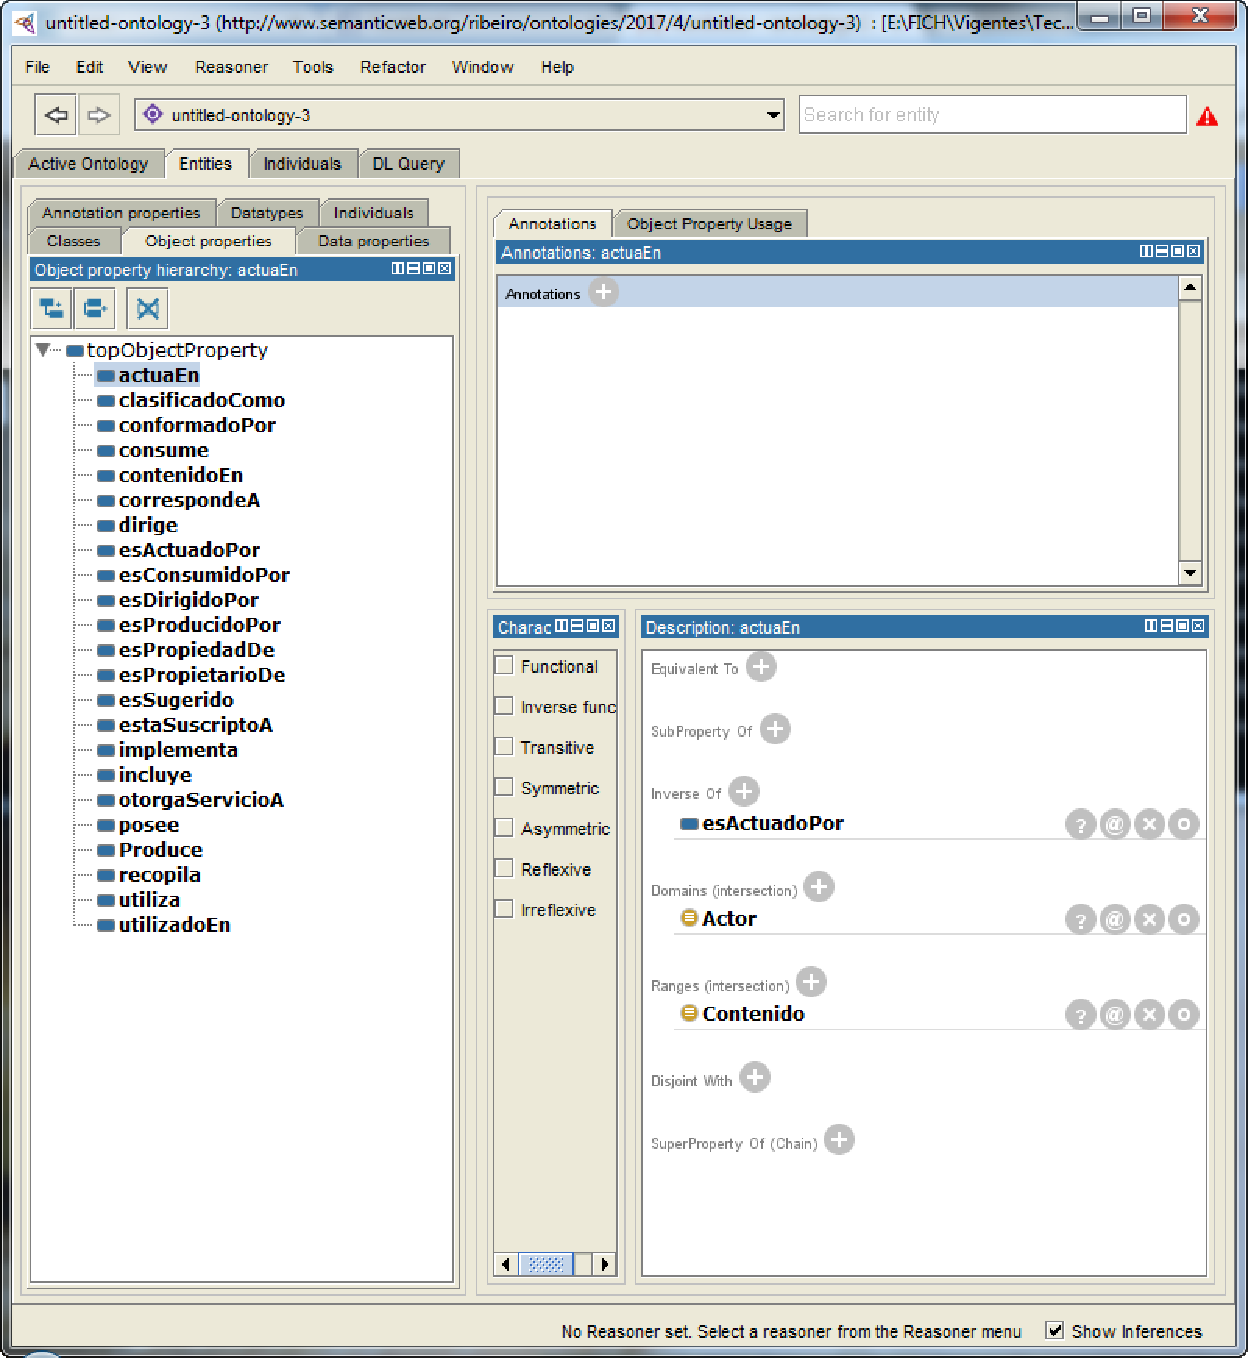
\includegraphics[width=\linewidth]{7}
\end{center}

\end{minipage}

\begin{minipage}{0.3\linewidth}

Una vez que se tiene la ontología finalmente implementada se puede utilizar el lenguaje de consultas SPARQL (derivado de RDQL) para realizar consultas sobre la misma.

\end{minipage} \hfill \begin{minipage}{0.65\linewidth}

\begin{center}
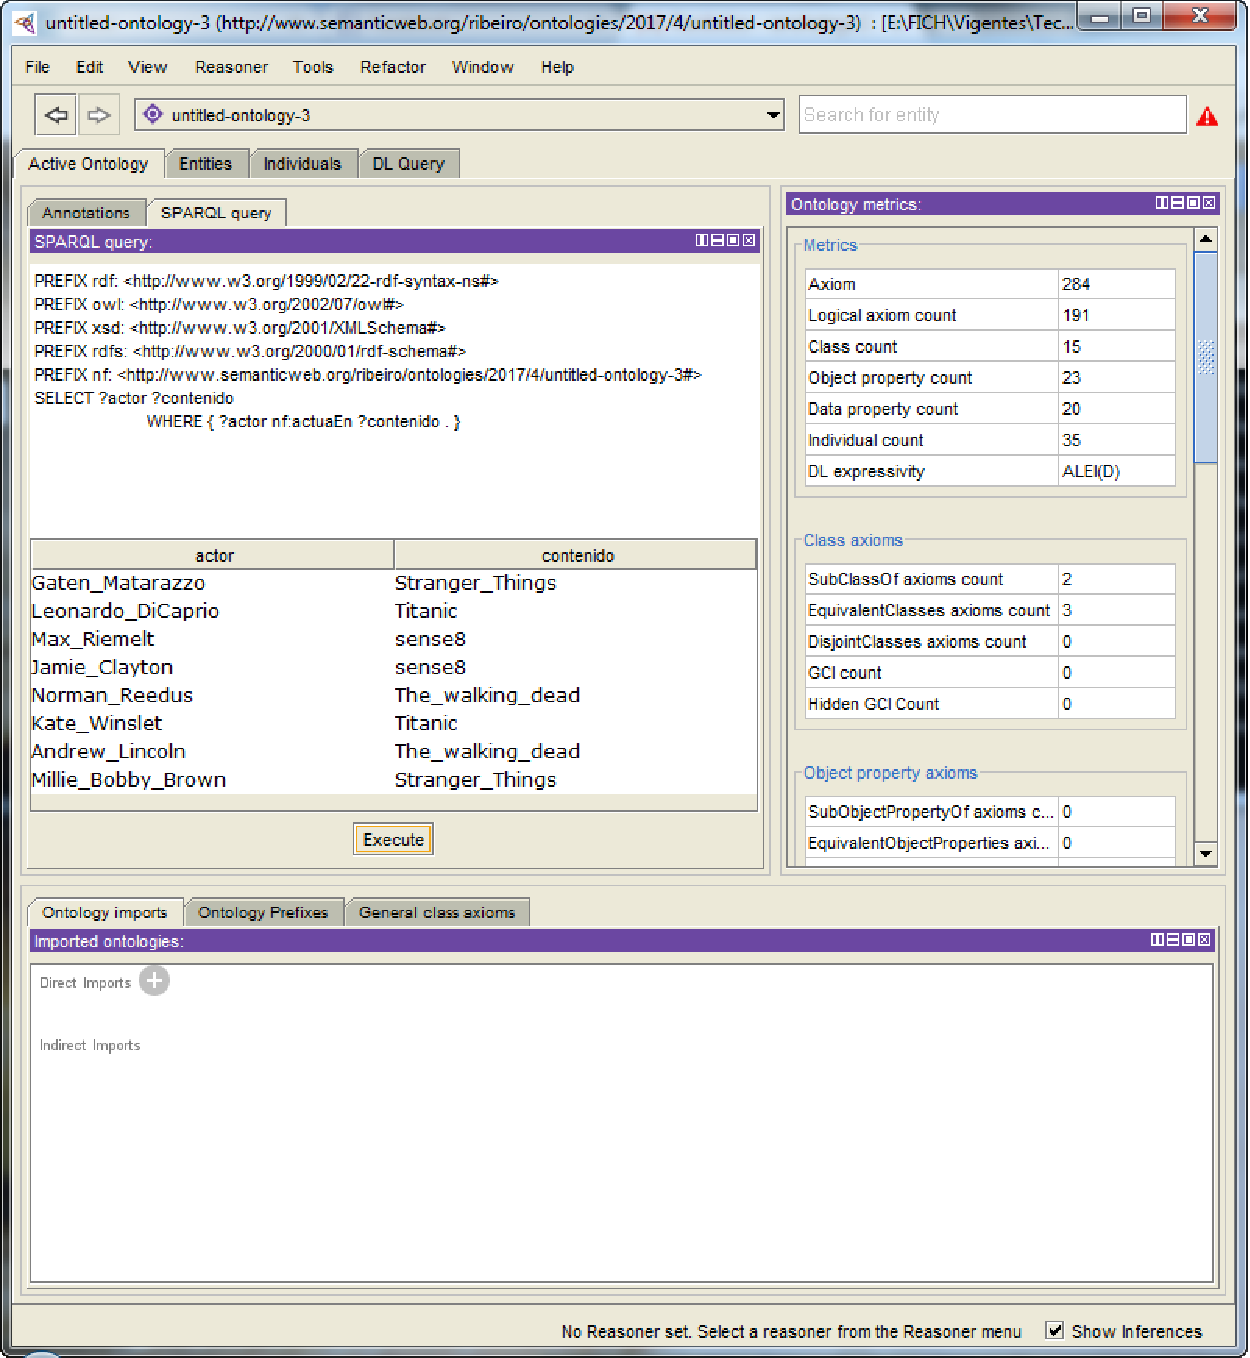
\includegraphics[width=\linewidth]{8}
\end{center}

\end{minipage}

\begin{thebibliography}{99}
\bibitem{SWP}
Grigoris Antoniou and Frank van Harmelen,
\emph{A Semantic Web Primer}, segunda edición.
The MIT Press, Cambridge, Massachusetts; London, England,
2008.
\end{thebibliography}

\end{document}